
%--------------- Chapter 5: Cluster Structure Stability ---------------%

\chapter{EFFICIENT CODEBOOK CONSTRUCTION}\label{Ch5:Grey Relational Analysis Based Codebook Construction}
\graphicspath{{Chapter5/Chapter5Figs/}{Chapter5/Chapter5Figs/}}

\section{Introduction}
\label{sec:1}

The codebook construction method using SBBO as discussed in Chapter \ref{Ch4:codebookconstruction} shows significant performance for the classification of histopathological images using the BOF method. However, these methods are computationally expensive. Moreover, it is observed that the GRA based keypoint selection method produces significant features due to effective GRG similarity measure and is computationally efficient as discussed in Chapter \ref{Ch3:GKS}. Therefore, in this chapter, a new Grey relational analysis based BOF method (GRA-BOF) is introduced which improves the efficiency of the codebook construction step of the standard BOF method. The method uses a Grey relational analysis for similarity measure in the clustering of the feature descriptors.



\section {Grey Relational Analysis based Bag-of-Features}\label{ch5:sec:GRABOF}

As discussed in Chapter \ref{Ch4:codebookconstruction}, K-means is not an efficient clustering method when applied on histopathological images having a large number of feature vectors. However, meta-heuristics based clustering methods show effective results but, they are not computationally efficient. Therefore, there is a need for a computationally efficient codebook construction method. 

The computational cost of K-means depends upon the distance calculations using Euclidean similarity measure. The size of the distance matrix is generally $O(n \times K)$, where, $n$ denotes feature count and $K$ denotes the number of visual words. For large $n$, the  Euclidean similarity becomes computationally expensive in terms of time and space. In literature, it has been proved that Grey relation analysis based similarity measure is computationally efficient than  Euclidean similarity \cite{chang2005} . Therefore, in this chapter, a new clustering algorithm has been introduced to find the most representative and relevant visual words in the BOF method. The overall flow of the new method is depicted in Figure \ref{fig:GRABOF} and a detailed description of the same is provided below.

\begin{figure}

\includegraphics[height=2.2in, width=6.5in]{codebook_GRA}
\caption[The GRA based BOF method]{\fontsize{10pt}{12pt}\selectfont  The GRA based BOF method}
\label{fig:GRABOF}
\end{figure}

\begin{enumerate}

\item Generate random training and validation sets from the histopathological image dataset.

\item Extract the features from training images to generate a set of feature descriptors ($X$) having $n$ features of $d$ dimensions as shown in Eq. (\ref{eq:Xaa})  
\begin{equation}\label{eq:Xaa}
X=\left\{\begin{array}{c}
x_{11} \  \ x_{12} \dots \ \    \dots \ \ x_{1d}\\ 
x_{21} \ \ x_{22}\dots  \ \     \dots \ \ x_{2d}\\
x_{31}  \ \ x_{32} \dots \ \    \dots \ \ x_{3d}\\
\dots \ \ \dots \ \    \dots \ \ \dots  \\
x_{n1} \ \ x_{n2} \dots \ \      \dots \ \ x_{nd}
\end{array}\right\}
\end{equation}

\item Calculate the mean of $X$ and find the feature vector which is nearby to the mean vector. Select this as a reference feature vector ($Ref$) which is considered as the first visual word and add this to the final codebook ($C$).

\item  All other feature vectors in $X$ are considered as the comparative sequences and similarity between all the comparative sequences with the reference sequence is measured using grey relational analysis. Grey relational similarity measure is a two-step process which is as follows:
\begin{itemize}
\item To measure the closeness between feature sequences a grey relational coefficient matrix ($\gamma$) is computed by using Eq. (\ref{eq:grc}).

\begin{equation} \label{eq:grc}
\gamma(Ref(d), X_{c}(d))=\frac{ \min \triangle(d) + \xi \max \triangle(d) }{\triangle(d)+\xi \max \triangle(d)}, 
\end{equation}
where, $ \triangle(d)= \mid Ref(d) - X_{c}(d) \mid$, for $c=1, \dots, \dots, n$ ($c\neq id(Ref)$), $d= 1, \dots , \dots, D$ and $\xi \in (0,1]$. $\xi$ is the random variable to control the variation between $ \min \triangle(d)$ and $\max\triangle(d)$. 

\item The GRC values are used to compute Grey relational grades (GRGs) which is given by Eq. (\ref{eq:grg})
\begin{equation} \label{eq:grg}
\Gamma(Ref, X_{c})= \sum_{d=1}^D[\alpha(d) \cdot \gamma(Ref(d), X_{c}(d))]
\end{equation}
where, $\alpha(d)$ is the weighting factor which  generally chooses  $\alpha_i(d) =1/p$ for all $D$. The values of GRC and GRG must always be between $0$ and $1$.
The resulting GRG vector is given by Eq. (\ref{eq:grgseq}).
\begin{equation}\label{eq:grgseq}
GRG=\left\{\begin{array}{c}g_{1} \\ 
g_{2} \\
g_{3}  \\
\dots   \\
g_{c} 
\end{array}\right\}
\end{equation}
where, $c=n-1$, and $GRG \in (0,1)$. Larger values of GRGs refer to the high similarity of the comparative sequence with the reference sequence.
\end{itemize}

\item Eliminate  $T\%$ comparative feature vectors having GRG  values close to $1$ because these features are more similar to the reference feature vector and are not relevant for the codebook construction. 

\item Update the set $X$ using Eq. (\ref{eq:Xup}) which only contains $m$ feature vectors   given by Eq. (\ref{ch5:eq:m}) 
\begin{equation}\label{ch5:eq:m}
m=n-\frac{n \times T}{100}
\end{equation}


\begin{equation}\label{eq:Xup}
X=\left\{\begin{array}{c}
x_{11} \  \ x_{12} \dots \ \    \dots \ \ x_{1d}\\ 
x_{21} \ \ x_{22}\dots  \ \     \dots \ \ x_{2d}\\
x_{31}  \ \ x_{32} \dots \ \    \dots \ \ x_{3d}\\
\dots \ \ \dots \ \    \dots \ \ \dots  \\
x_{m1} \ \ x_{m2} \dots \ \      \dots \ \ x_{md}
\end{array}\right\}
\end{equation} 

\item Repeat Step 3 to 6 until only one feature is left in $X$.

\item The updated set $C$ in step 3 is considered as the cluster centers or visual words.

\item Represent each image in the training set in the histogram of these visual words.

\item Give the histogram along with the corresponding annotations to the SVM classifier for training.

\item Pick any image from the validation set and represent it into the histogram in the same way as discussed above and feed it to SVM for predicting its label.  

\end{enumerate}

The process of clustering algorithm using GRA is also given in Algorithm \ref{algo:KSGRA}. 

\begin{algorithm}
\caption{The GRA based clustering method}
\label{algo:KSGRA}
\footnotesize
 \setstretch{1.4}
\begin{algorithmic}
\STATE \textbf{Input:}  A set of feature vectors, known as descriptor $D$, having $n$  strong feature vectors and a cut-off threshold ($T$)  
\STATE \textbf{Output:}  Reduced descriptor $S$ having $m$ feature vectors ($m<n$)
\WHILE  {($size(D)>1$)}
     \STATE Select a reference vector ($R$) near to the mean of $D$ ;
     \STATE $D= D- R$
      \STATE Calculate GRGs for each feature vector in $D$ with $R$ (Eq. (\ref{eq:grg}));
    \STATE Sort the $D$ according the GRG values in descending order and delete the first $T\%$ feature vectors from $D$ ;
    \STATE Update vector $S=[S\ \ R]$ ;
\ENDWHILE \\
\STATE The resulting set $S$ is considered as the cluster centers or visual words.
\end{algorithmic}
\end{algorithm}

\section{Experimental Results} \label{Sec:exp}

The efficacy of the GRA-BOF method against other considered state-of-the-art methods, it has been tested on ADL and Blue histology histopathological image datasets. For comparative analysis, two BOF based classification methods, standard BOF and IKS2-BOF and three state-of-the-art classification methods, SVM, SRC, and SHIRC, have been considered. A brief description of these methods is provided below.

\begin{itemize}
\item \emph{IKS2-BOF:} Iterative keypoints selection methods \cite{lin2016} reduce the complexity of vector quantization in the BOF method by selecting some representative keypoints from the images. The representative keypoints can be generated either randomly (IKS1) or using K-means (IKS2). The performance of the IKS2-BOF classification method is better than the IKS1-BOF method on natural image datasets. Hence, in this chapter, the IKS2-BOF method is considered and evaluated on the histopathological image dataset for the comparative analysis against the new method.  The parameter settings for the simulation is taken from the respective literature. 

\item \emph{SVM:} SVM is one the state-of-the-art classification method discussed by Srinivas et. al \cite{srinivas2014}. It extracts the features using a well-known feature extraction method for histopathological images, namely WND-CHARM \cite{orlov2008} and classification, support vector machine is used.  The simulation results for this method on the ADL dataset is taken from Srinivas et al. \cite{srinivas2014}.

\item \emph{SRC:} Sparse representation  based classification methods are initially used for face recognition applications\cite{Wagner2012}.After that, it is also widely used in medical images \cite{srinivas2014}. It is a single luminance channel based sparse representation of RGB images which is further used for classification. The simulation results for this method on the ADL dataset is taken from \cite{srinivas2014}.

\item \emph{SHIRC:} SHIRC is the multi-channel sparsity model which is an extension of the standard SRC approach for three color channels. It is used for the classification of histopathological images. The simulation results for this method on the ADL dataset is taken from Srinivas et al. \cite{srinivas2014}.
\end{itemize}

\begin{figure}[ht!]
\centering
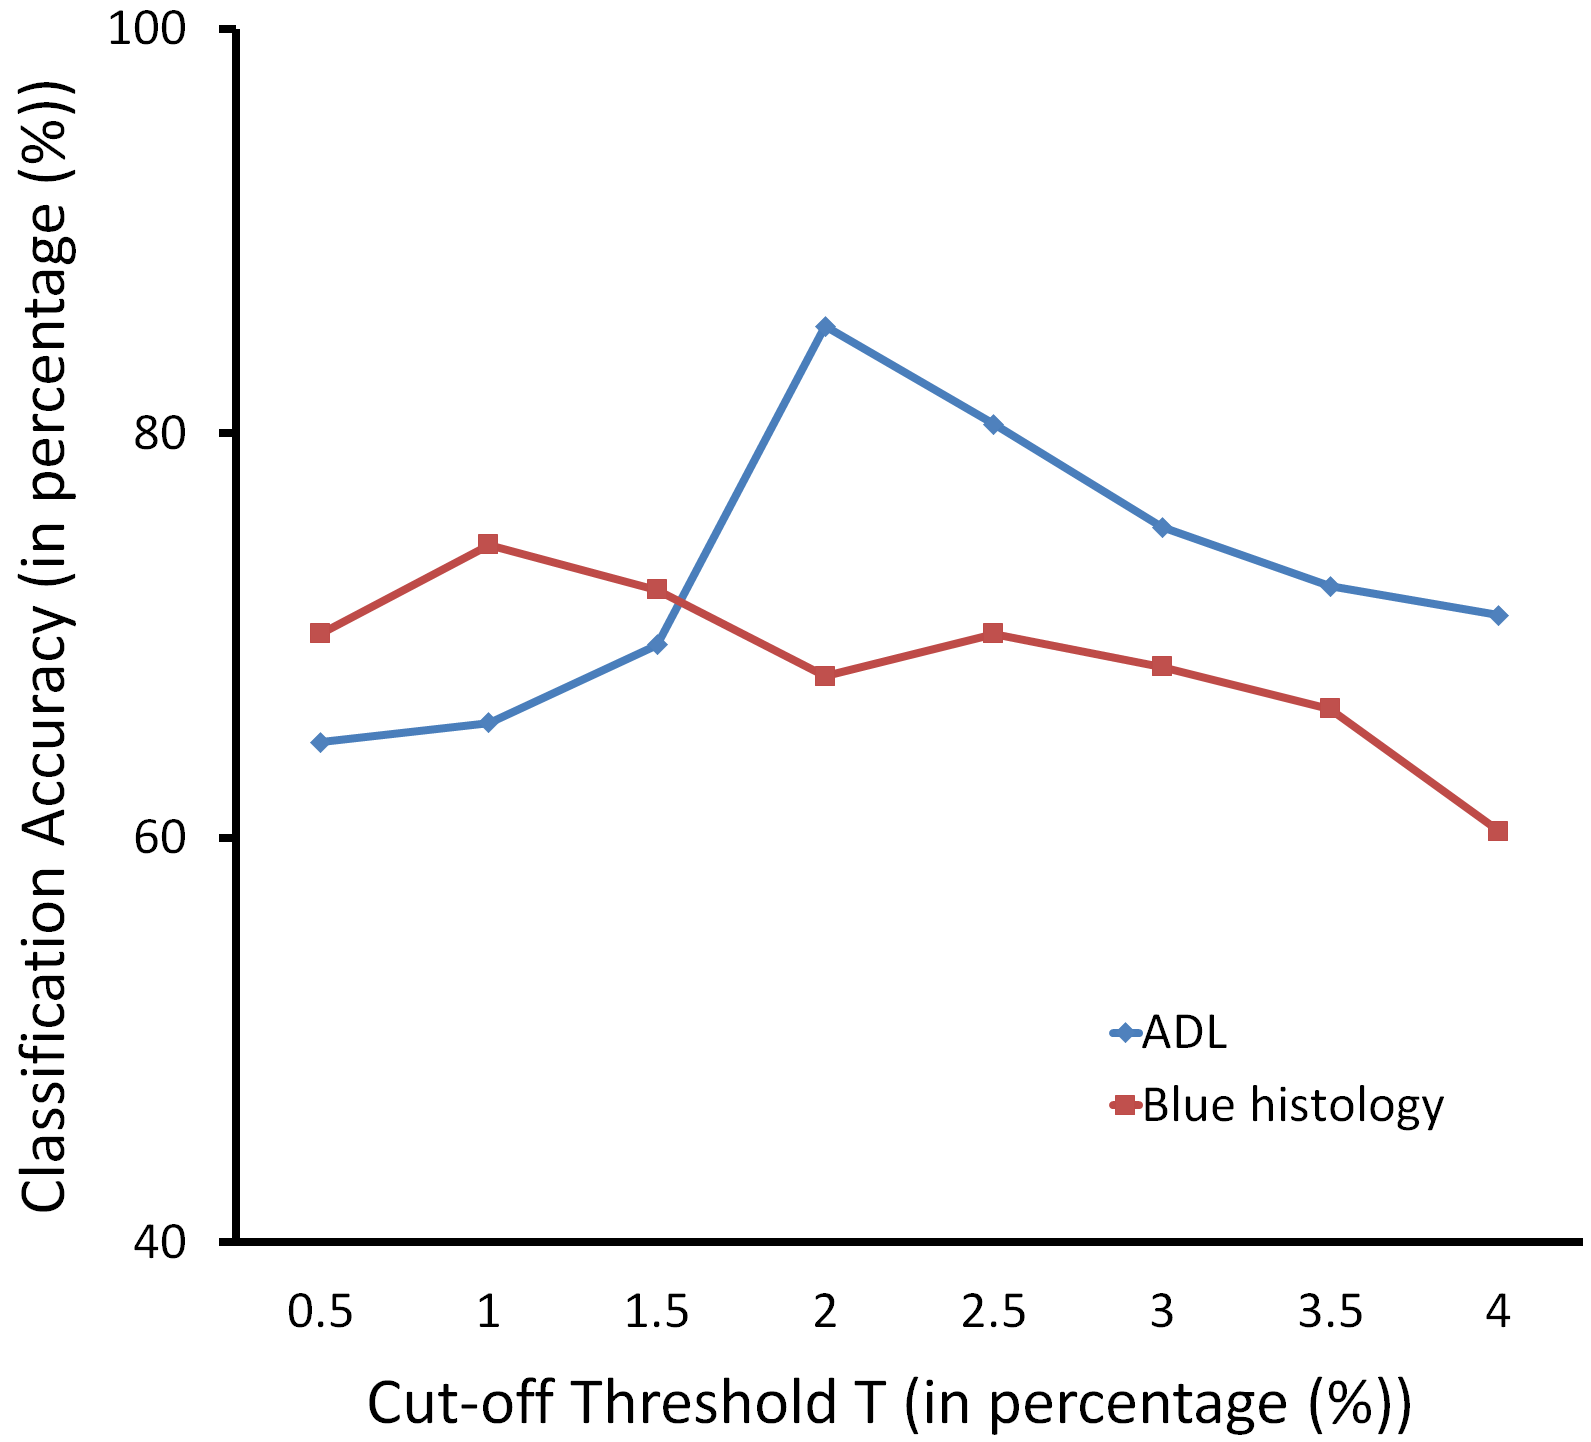
\includegraphics[scale=0.2]{emp}
\caption[Impact analysis of cut-off threshold value over classification accuracy on ADL and Blue histology datasets]{\fontsize{10pt}{12pt}\selectfont Impact analysis of cut-off threshold ($T$) value over classification accuracy on ADL and Blue histology datasets}
\label{ch5:fig:T3}
\end{figure}
 The main parameter in the GRA-BOF is the cut-off threshold ($T$) which is used to eliminate similar points. Figure \ref{ch5:fig:T3} shows the classification accuracy obtained by the GRA-BOF method using SVM on ADL and Blue histology datasets. From the figure, it can be observed that for different values of cut-off thresholds there is a slight variation in the obtained accuracy over each dataset. From the results, the cut-off threshold is taken $2\%$ for  ADL histopathological dataset while for blue histology dataset $1\%$ cut-off threshold value is considered. Moreover, the new GRA-BOF method uses SVM for the classification with $10$-fold cross-validation to overcome the issue of over-fitting. The selection of appropriate kernel function is very important, therefore $\chi^2$ RBF kernel is used in this chapter as it shows better performance in Lin et. al \cite{lin2016}. For each trial, the images for training and validation sets are randomly selected from the dataset. 
 
\begin{table}[h]
\centering
\caption[Confusion matrix generated by considered methods on ADL histopathological image dataset]{\fontsize{10pt}{12pt}\selectfont Confusion matrix generated by considered methods on ADL histopathological image dataset}
    \label{ch5:tab:cm}
\renewcommand{\arraystretch}{1.2}
{\scriptsize 
\begin{tabular}{|c|c|c|c|c|c|c|c|}
\hline
&  & \multicolumn{2}{c|}{Kidney}& \multicolumn{2}{c|}{Lung} & \multicolumn{2}{c|}{Spleen}\\
\cline{3-8}
Class &Method & Normal  & Inflamed & Normal  & Inflamed & Normal  & Inflamed\\
\hline
&SVM& 0.69 & 0.28 & 0.89 & 0.37 & 0.51 & 0.13 \\
&SRC & 0.88&0.25&0.73&0.24&0.71&0.21\\
Normal &SHIRC &0.82&0.17&0.75&0.15&0.65&0.12\\
&BOF&0.82&0.31&0.72&0.25&0.55&0.23\\
&IKS2&0.85&0.23&0.83&0.30&0.68&0.13\\
&GRA-BOF&\textbf{0.89}&0.09&\textbf{0.92}&0.06&\textbf{0.75}&0.11\\
\hline

&SVM& 0.31&0.72&0.11&0.62&0.49&0.87\\
&SRC&0.13&0.75&0.27&0.78&0.29&0.79\\
Inflamed &SHIRC&0.18&0.83&0.25&0.85&0.35&0.88\\
&BOF&0.18&0.69&0.28&0.75&0.45&0.77\\
&IKS2&0.15&0.77&0.17&0.7&0.32&0.87\\
&GRA-BOF&0.11&\textbf{0.91}&0.08&\textbf{0.94}&0.25&\textbf{0.89}\\

\hline
\end{tabular}
}
\end{table}

\begin{figure}[h]
\centering
\subfigure[]{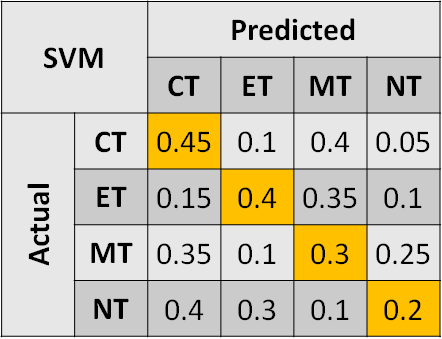
\includegraphics[width=0.3\linewidth]{CM_SVM_Tissue}}
\subfigure[]{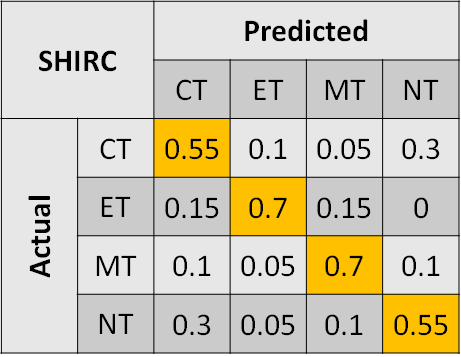
\includegraphics[width=0.3\linewidth]{CM_SHIRC_Tissue}} 
\subfigure[]{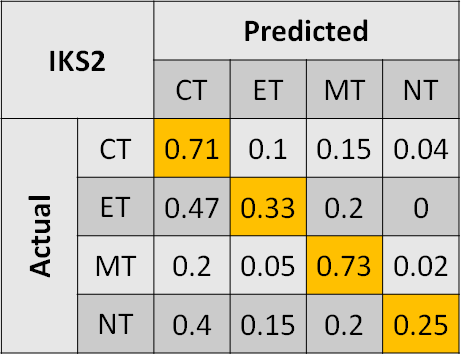
\includegraphics[width=0.3\linewidth]{CM_IKS2_Tissue}}
\subfigure[]{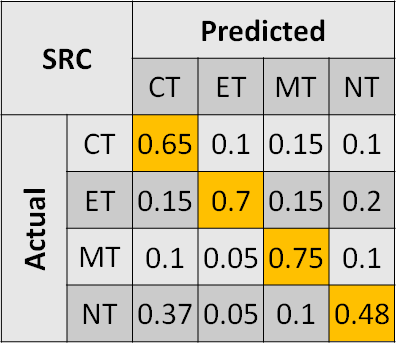
\includegraphics[width=0.3\linewidth]{CM_SRC_Tissue}}
\subfigure[]{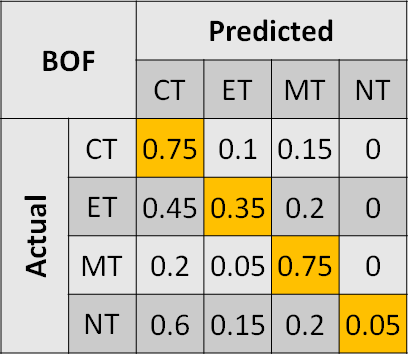
\includegraphics[width=0.3\linewidth]{CM_BOF_Tissue}}
\subfigure[]{\includegraphics[width=0.3\linewidth]{CM_GRABOF_Tissue}}
 \caption[Confusion matrices returned by SVM, SRC, SHIRC, BOF, IKS2, and GRA-BOF on Blue histology image dataset]{\fontsize{10pt}{12pt}\selectfont  Confusion matrices returned by (a) SVM, (b) SRC, (c) SHIRC, (d)BOF, (e)IKS2 (f) GRA-BOF on Blue histology image dataset}
\label{ch5:fig:CM_tissue}
\end{figure}

The statistics of the classification performance are presented by the confusion matrices returned by each method to classify each organ image. These confusion matrices are shown in Table \ref{ch5:tab:cm}  for kidney, lung, and spleen of ADL histopathological image datasets. The rows of the confusion matrices represent the predicted output of the classifier and columns refer to the actual class of the test images.  The confusion matrices show the average results achieved from $10$ trials. Figure \ref{ch5:fig:CM_tissue} shows the confusion matrices returned by each method on blue histology image dataset.  From Table \ref{ch5:tab:cm} and Figure \ref{ch5:fig:CM_tissue},  it can be observed that SVM, trained directly on features extracted by the WND-CHARM method, does not perform well for any of the classes. It means the relevant features are not used for training. The performance of other state-of-the-art methods is far better than this method.  The performance of the GRA-BOF method is tremendous in identifying the images of all the classes more accurately. It identifies almost all the inflamed lung images from the ADL dataset while the worst performance is observed in the case of the normal spleen image class which is also the best as compared to other methods. While, in the case of blue histology dataset, the GRA-BOF method identifies all four types of tissues in a more efficient manner as compared to other considered methods. 

In medical image classification, pathologists are more interested in true negatives (i.e., the accuracy of identifying the inflamed images correctly). It can be illustrated from Table \ref{ch5:tab:cm} that the GRA-BOF method identifies the inflamed test images more accurately than other considered competitive methods with the accuracy of $91\%$, $94\%$, and $89\%$ for kidney, lung, and spleen organs respectively. Moreover, it also maintains high classification accuracy to categorize normal test images. The GRA-BOF method classifies the inflamed tissue images of each organ much more accurately than normal tissue images. Hence, the probability of normal image wrongly identified as the inflammatory image (i.e., false alarm rate) is very less for the new method while SRC, BOF, and IKS2 have high false alarm rates on kidney images. Moreover, SVM and IKS2 also show the high false alarm rates for lung organ images. The false negatives to detect the disease is comparatively higher in the case of the GRA-BOF (91.3\%) method which is the most relevant metric for the pathologists. For the blue histology image dataset, it can be observed from the Figure \ref{ch5:fig:CM_tissue} that the GRA-BOF method returns highest true positives for the identification of all the tissue types. However, the identification of nervous tissue image is a challenging task due to the variety of staining used in it. The GRA-BOF method identifies the nervous tissue test image with an accuracy of $65\%$ while the identification rate of other considered methods for nervous tissue is below $50\%$ except SHIRC. Moreover, for connective and epithelial tissues, the GRA-BOF method identifies $80\%$ and $78\%$ of test images receptively. Therefore, from the study of confusion matrices returned by all the classification methods, it can be stated that the GRA-BOF method shows consistent and the best results for all the considered organ images.   

\begin{table}[h]
\centering
\caption[Classification performance with other methods based on recall, specificity, precision, FPR, and accuracy]{\fontsize{10pt}{12pt}\selectfont Classification performance with  other methods based on  recall, specificity, precision, FPR, and accuracy on ADL dataset}
    \label{ch5:tab:adlp}
\renewcommand{\arraystretch}{1.2} 
{\scriptsize
\begin{tabular}{|c|c|c|c|c|c|c|}
\hline
    Organ &    Algorithms    &    Recall    &Specificity    &Precision    &    FPR    &    Accuracy    \\
\hline
    &    SVM    &    0.69    &    0.72    &    0.71    &    0.28    &    0.71    \\
    &    SRC    &    0.88    &    0.75    &    0.78    &    0.25    &    0.81    \\
    &    SHIRC    &    0.83    &    0.83    &    0.83    &    0.17    &    0.83    \\
Kidney    &    BOF    &    0.82    &    0.69    &    0.73    &    0.31    &    0.76    \\
    &    IKS2-BOF    &    0.85    &    0.77    &    0.79    &    0.23    &    0.81    \\
    &    GRA-BOF    &\textbf{    0.89    }&\textbf{    0.91    }&\textbf{    0.91    }&\textbf{    0.09    }&\textbf{    0.90    }\\
\hline    
&    SVM    &    0.89    &    0.63    &    0.70    &    0.37    &    0.76    \\
    &    SRC    &    0.73    &    0.76    &    0.75    &    0.24    &    0.75    \\
    &    SHIRC    &    0.75    &    0.85    &    0.83    &    0.15    &    0.80    \\
Lung    &    BOF    &    0.72    &    0.75    &    0.74    &    0.25    &    0.74    \\
    &    IKS2-BOF    &    0.83    &    0.70    &    0.73    &    0.30    &    0.77    \\
    &    GRA-BOF    &\textbf{    0.92    }&\textbf{    0.94    }&\textbf{    0.94    }&\textbf{    0.06    }&\textbf{    0.93    }\\
\hline    
&    SVM    &    0.51    &    0.87    &    0.80    &    0.13    &    0.69    \\
    &    SRC    &    0.71    &    0.79    &    0.77    &    0.21    &    0.75    \\
    &    SHIRC    &    0.65    &    0.88    &    0.85    &    0.12    &    0.77    \\
Spleen    &    BOF    &    0.55    &    0.77    &    0.71    &    0.23    &    0.66    \\
    &    IKS2-BOF    &    0.68    &    0.87    &    0.84    &    0.13    &    0.78    \\
    &    GRA-BOF    &\textbf{    0.75    }&\textbf{    0.89    }&\textbf{    0.87    }&\textbf{    0.11    }&\textbf{    0.82    }\\
\hline
\end{tabular}
}
\end{table}

\begin{table}[h]
\centering
\caption[Classification performance  with  other methods based on  recall, precision, F1 score, specificity, and average accuracy on Blue histology dataset]{\fontsize{10pt}{12pt}\selectfont Classification performance  with  other methods based on  recall, precision, F1 score, specificity, and average accuracy on Blue histology dataset}
    \label{ch5:tab:tissuep}
{\scriptsize
\renewcommand{\arraystretch}{1.2} 
\begin{tabular}{|c|l|c|c|c|c|c|c|}
\hline
Categoty    &    Parameters    &    SVM    &    SRC    &    SHIRC    &    BOF    &    IKS2    &    GRA-BOF    \\
\hline
    &    Recall    &    0.450    &    0.650    &    0.550    &    0.750    &    0.710    &    \textbf{0.800    }\\
    &    Precision    &    0.512    &    0.512    &    0.500    &    0.375    &    0.399    &    \textbf{0.696}    \\
CT    &    F1 Score     &    0.573    &    0.573    &    0.524    &    0.500    &    0.511    &    \textbf{0.744    }\\
    &    Specificity    &    0.806    &    0.806    &    0.814    &    0.583    &    0.643    &    \textbf{0.883    }\\
    \hline
    &    Recall    &    0.400    &    0.583    &    0.700    &    0.350    &    0.330    &    \textbf{0.780    }\\
    &    Precision    &    0.778    &    0.778    &    0.778    &    0.538    &    0.524    &    \textbf{0.650    }\\
ET    &    F1 Score     &    0.667    &    0.667    &    0.737    &    0.424    &    0.405    &\textbf{    0.709    }\\
    &    Specificity    &    0.933    &    0.933    &    0.932    &    0.900    &    0.900    &    \textbf{0.860}    \\
    \hline
    &    Recall    &    0.300    &    0.750    &    0.737    &    0.750    &    0.730    &\textbf{    0.751    }\\
    &    Precision    &    0.652    &    0.652    &    0.700    &    0.577    &    0.570    &    \textbf{0.815}    \\
MT    &    F1 Score     &    0.698    &    0.698    &    0.718    &    0.652    &    0.640    &    \textbf{0.781    }\\
    &    Specificity    &    0.875    &    0.875    &    0.900    &    0.817    &    0.817    &\textbf{    0.943}    \\
    \hline
    &    Recall    &    0.200    &    0.480    &    0.550    &    0.050    &    0.250    &    \textbf{0.650    }\\
    &    Precision    &    0.545    &    0.545    &    0.579    &    1.000    &    0.806    &\textbf{    0.890}    \\
NT    &    F1 Score     &    0.511    &    0.511    &    0.564    &    0.095    &    0.382    &\textbf{    0.751    }\\
    &    Specificity    &    0.875    &    0.875    &    0.864    &    1.000    &    0.980    &    \textbf{0.973}    \\
    \cline{2-8}
    &    Average Accuracy    &    33.8    &    61.4    &    63.3    &    47.5    &    50.5    &\textbf{    74.5    }\\

\hline
\end{tabular}
}
\end{table}

Moreover, the various performance parameters are used to analyze the efficacy of the GRA-BOF method such as recall, specificity, precision, false positive rate (FPR), and accuracy. Table \ref{ch5:tab:adlp} depicts the computed values of these parameters on the kidney, lung, and spleen datasets while Table \ref{ch5:tab:tissuep} shows the results for blue histology dataset. From the tables, it can be stated that the GRA-BOF method outperforms other methods over recall, specificity, precision, recall, FPR, and accuracy. The classification accuracies of the GRA-BOF on kidney, lung, and spleen datasets are  90\%, 93\%, and 82\% respectively which is higher than the other considered state-of-art methods. The overall accuracy on the ADL dataset is 88.3\% which is better than other considered methods. Further, the average classification accuracy of the GRA-BOF method on the blue histology dataset is $74.5\%$, which is highest among other considered methods.


Moreover, a comparison of the F1 score, G-mean, sensitivity, and specificity is represented using the radar chart in Figure \ref{ch5:fig:radar}. The radar chart shows that the method with the largest area and symmetrical shape performs better than other. From the figure, it can be illustrated that the GRA-BOF method shows better results than all other methods. These results validate that the efficacy of the GRA-BOF method for histopathological image classification.
\begin{figure}[t]
\centering
\subfigure[Spleen]{\includegraphics[width=0.3\linewidth]{spleen_radar}}
\subfigure[ Kidney]{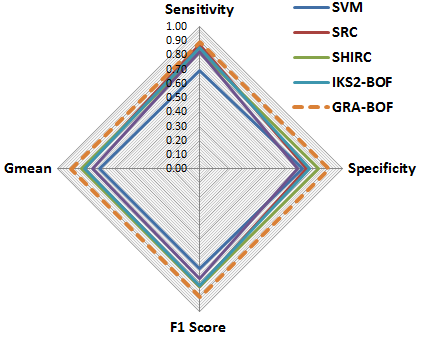
\includegraphics[width=0.3\linewidth]{kidney_radar}}
\subfigure[Lung]{\includegraphics[width=0.3\linewidth]{lung_radar}} 
 \caption[Radar chart for average results on Spleen dataset, Kidney dataset, and Lung dataset]{\fontsize{10pt}{12pt}\selectfont Radar chart for average results on (a) Spleen dataset, (b) Kidney dataset, and (c) Lung dataset}
\label{ch5:fig:radar}
\end{figure}

\section{Summary}\label{sec:con}

This chapter introduced a new Grey relational analysis based BOF method (GRA-BOF) which improves the efficiency of the codebook construction phase of the standard BOF method. The method uses a Grey relational analysis for similarity measure in the codebook construction phase of BOF. The GRA-BOF method has been validated on three datasets, Kidney, Lung, and Spleen of ADL histopathological image dataset along with the blue histology tissue image dataset. The average accuracy of the GRA-BOF method is $88.3\%$ and $74.5\%$ on ADL and Blue histology datasets respectively which are the highest among other state-of-the-art methods. The classification results of the GRA-BOF method has also been analyzed using confusion matrix, precision, recall, G-mean, F1 score, and radar charts. The experimental results validate that the GRA-BOF method outperforms the other considered methods for histopathological image classification. 

The next chapter discusses the vector quantization phase of BOF and presents a new efficient vector quantization method in the BOF framework.